\documentclass[12pt,letterpaper]{article}
\usepackage{amsmath}
\usepackage{amsfonts}
\usepackage{amsthm}
\usepackage{mathtools}
\usepackage{cancel}
\usepackage[margin=1in]{geometry}
\usepackage{titling}
\usepackage{fp}
\usepackage{enumitem}
\usepackage[super]{nth}
\usepackage{dcolumn}
\usepackage{minted}
\usepackage[title]{appendix}
\usepackage{pgfplots}
\pgfplotsset{compat=1.8}
\usepgfplotslibrary{statistics}
\usepackage[round-mode=figures,round-precision=3,scientific-notation=false]{siunitx}

\newcolumntype{d}{D{.}{.}{-1}}

\setlength{\droptitle}{-10ex}

\preauthor{\begin{flushright}\large \lineskip 0.5em}
\postauthor{\par\end{flushright}}
\predate{\begin{flushright}\large}
\postdate{\par\end{flushright}}

\title{STA 032 R Homework 5\vspace{-2ex}}
\author{Hardy Jones\\
        999397426\\
        Professor Melcon\vspace{-2ex}}
\date{Winter 2015}

\begin{document}
  \maketitle

  \newmintedfile[rData]{r}{ fontsize=\footnotesize
                          , frame=single
                          }

  \begin{enumerate}
    \item
      \begin{enumerate}
        \item \num{0.1098132}
        \item \num{0.07457804}
        \item \num{0.05509422}
        \item \num{2.955362e-10}
      \end{enumerate}
    \item
      \begin{enumerate}
        \item \num{0.005886852}
        \item \num{0.00845186}
        \item \num{0.005387753}
        \item \num{2.959784e-10}
      \end{enumerate}
    \item
      \begin{enumerate}
        \item
          The mean of the uncorrected column is \num{3.450677e-02}.

          The mean of the corrected column is \num{4.776026e-05}.

        \item
          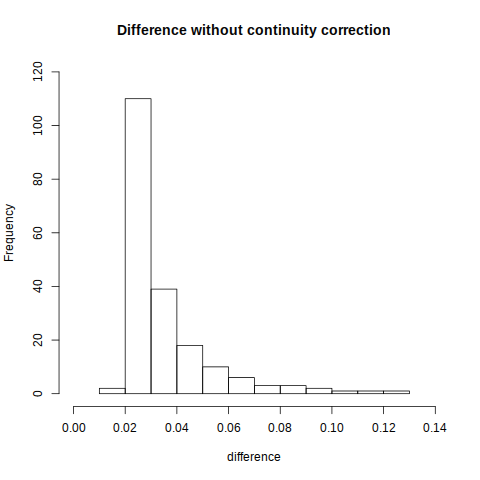
\includegraphics[width=\linewidth/2-10pt]{prob3b1.png}
          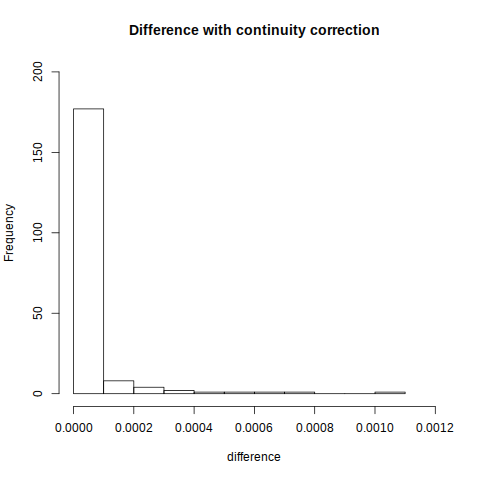
\includegraphics[width=\linewidth/2-10pt]{prob3b2.png}

        \item
          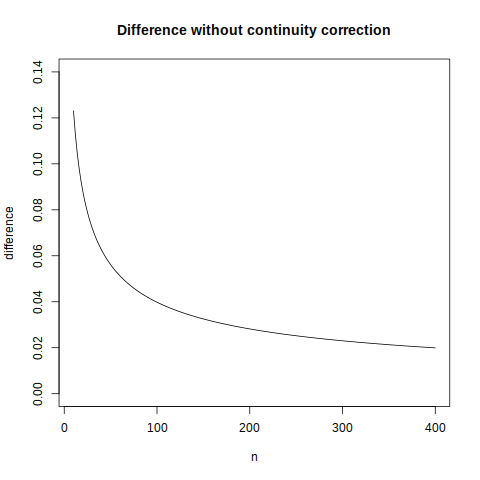
\includegraphics[width=\linewidth/2-10pt]{prob3c1.png}
          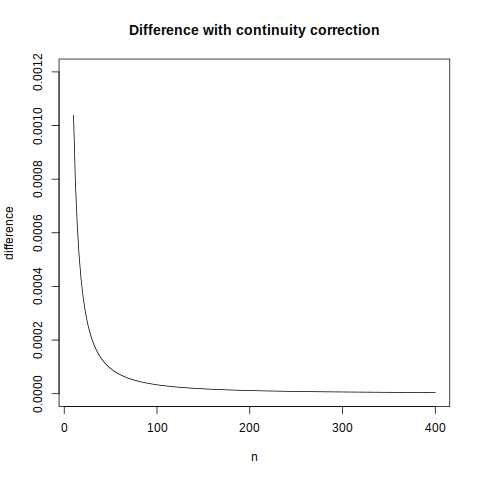
\includegraphics[width=\linewidth/2-10pt]{prob3c2.png}

        \item
          Yes, I think implementing the continuity correction is worthwhile if you are approximating a binomial probability with a normal distribution.

          The additional complexity to compute the correction is a constant factor. So, when using the correction, the difference in computation time is not noticeable. However, the results are non-trivial.

          In the above example, the correction provided a better approximation at all values of $n$ than any uncorrected approximation at any $n$.

      \end{enumerate}
  \end{enumerate}

  \begin{appendices}
    \section{R code}

        \subsection*{Problem 1}
            \rData{prob1.R}
            \subsubsection*{(a)}
                \rData{prob1a.R}
            \subsubsection*{(b)}
                \rData{prob1b.R}

        \subsection*{Problem 2}
            \rData{prob2.R}
            \subsubsection*{(a)}
                \rData{prob2a.R}
            \subsubsection*{(b)}
                \rData{prob2b.R}

        \subsection*{Problem 3}
            \rData{prob3.R}
            \subsubsection*{(a)}
                \rData{prob3a.R}
            \subsubsection*{(b)}
                \rData{prob3b.R}

\end{appendices}


\end{document}
